\documentclass[aspectratio=169,10pt]{beamer}

\usepackage{fontspec}
\usepackage{booktabs}
\usepackage{graphicx}
\usepackage{array}
\usepackage{xcolor}
\usepackage{tikz}
\usepackage{amsmath}

\IfFontExistsTF{Arial}{
  \setsansfont{Arial}
}{
  \setsansfont{TeX Gyre Heros}
}
\renewcommand{\familydefault}{\sfdefault}

\definecolor{OffWhite}{HTML}{FAFAFA}
\definecolor{Accent}{HTML}{4F46E5}
\definecolor{Ink}{HTML}{111827}
\definecolor{Muted}{HTML}{6B7280}
\definecolor{Line}{HTML}{E5E7EB}

\setbeamertemplate{navigation symbols}{}
\setbeamertemplate{headline}{}
\setbeamertemplate{blocks}[default]
\setbeamertemplate{itemize item}{\raisebox{0.18ex}{\scriptsize\textcolor{Accent}{\textbullet}}}
\setbeamertemplate{itemize subitem}{\raisebox{0.18ex}{\tiny\textcolor{Accent}{\textbullet}}}
\setbeamertemplate{enumerate item}{\textcolor{Accent}{\insertenumlabel.}}
\setbeamertemplate{footline}{
  \leavevmode%
  \hbox{%
    \begin{beamercolorbox}[wd=.50\paperwidth,ht=3.0ex,dp=1.4ex,leftskip=0.72cm]{footline}%
      \textcolor{Muted}{STAT GR5293 Final Project}
    \end{beamercolorbox}%
    \begin{beamercolorbox}[wd=.50\paperwidth,ht=3.0ex,dp=1.4ex,rightskip=0.72cm plus1fil]{footline}%
      \hfill\textcolor{Muted}{\insertframenumber\,/\,\inserttotalframenumber}
    \end{beamercolorbox}%
  }%
}
\setbeamertemplate{frametitle}{
  \vspace{0.25cm}
  {\usebeamerfont{frametitle}\insertframetitle\par}
  \vspace{0.08cm}
}

\setbeamercolor{background canvas}{bg=OffWhite}
\setbeamercolor{normal text}{fg=Ink,bg=OffWhite}
\setbeamercolor{frametitle}{fg=Ink,bg=OffWhite}
\setbeamercolor{title}{fg=Ink}
\setbeamercolor{structure}{fg=Accent}
\setbeamercolor{footline}{fg=Muted,bg=OffWhite}

\setbeamerfont{title}{size=\fontsize{29}{33}\selectfont,series=\bfseries}
\setbeamerfont{subtitle}{size=\fontsize{16}{22}\selectfont,series=\mdseries}
\setbeamerfont{author}{size=\fontsize{13}{18}\selectfont}
\setbeamerfont{institute}{size=\fontsize{12}{16}\selectfont}
\setbeamerfont{date}{size=\fontsize{12}{16}\selectfont}
\setbeamerfont{frametitle}{size=\fontsize{32}{36}\selectfont,series=\bfseries}
\setbeamerfont{normal text}{size=\fontsize{18}{25}\selectfont}
\setbeamerfont{itemize/enumerate body}{size=\fontsize{18}{25}\selectfont}
\setbeamerfont{itemize/enumerate subbody}{size=\fontsize{15}{21}\selectfont}

\setbeamersize{text margin left=0.72cm,text margin right=0.72cm}

\newcommand{\protocol}[1]{\texttt{#1}}
\newcommand{\hl}[1]{\textcolor{Accent}{#1}}
\newcommand{\smallmuted}[1]{{\fontsize{11}{15}\selectfont\textcolor{Muted}{#1}}}
\newcommand{\bodytext}[1]{{\fontsize{18}{24}\selectfont #1}}
\newcommand{\compacttext}[1]{{\fontsize{14}{18}\selectfont #1}}
\newcommand{\stat}[3]{%
  \begin{minipage}[t]{0.30\textwidth}
    {\fontsize{28}{32}\selectfont\bfseries\textcolor{Accent}{#1}}\par
    \vspace{0.05cm}
    {\fontsize{13}{17}\selectfont\textcolor{Ink}{#2}}\par
    \vspace{0.04cm}
    {\fontsize{10}{14}\selectfont\textcolor{Muted}{#3}}
  \end{minipage}
}
\newcommand{\sidestat}[3]{%
  \begin{minipage}[t]{\linewidth}
    {\fontsize{25}{29}\selectfont\bfseries\textcolor{Accent}{#1}}\par
    \vspace{0.04cm}
    {\fontsize{13}{17}\selectfont\textcolor{Ink}{#2}}\par
    \vspace{0.03cm}
    {\fontsize{10}{14}\selectfont\textcolor{Muted}{#3}}
  \end{minipage}
}
\newcommand{\divider}{\vspace{0.18cm}{\color{Line}\hrule height 0.6pt}\vspace{0.28cm}}
\newcommand{\sectionlabel}[1]{{\fontsize{11}{15}\selectfont\bfseries\textcolor{Accent}{#1}}\par\vspace{0.10cm}}

\title{Communication Protocol Effects on\\ Multi-Agent System Efficiency\\ and Task Completion}
\subtitle{Final Project Presentation}
\author{Yi Zhang \quad Xian Zhang \quad Tianyu Zhan}
\institute{Department of Statistics, Columbia University}
\date{Spring 2026}

\begin{document}

\begin{frame}[plain]
  \vspace{0.35cm}
  \sectionlabel{STAT GR5293}
  {\usebeamerfont{title}\inserttitle\par}
  \vspace{0.22cm}
  {\usebeamerfont{subtitle}\textcolor{Muted}{\insertsubtitle}\par}
  \vfill
  {\usebeamerfont{author}\insertauthor\par}
  \vspace{0.08cm}
  {\usebeamerfont{institute}\textcolor{Muted}{\insertinstitute}\par}
  \vspace{0.08cm}
  {\usebeamerfont{date}\textcolor{Muted}{\insertdate}\par}
  \vspace{0.35cm}
  {\color{Accent}\rule{2.8cm}{1.2pt}}
\end{frame}

\begin{frame}{Rubric Map}
  \sectionlabel{FINAL PRESENTATION, 30\%}
  \begin{columns}[T,onlytextwidth]
    \begin{column}{0.31\textwidth}
      {\fontsize{22}{27}\selectfont\bfseries Problem}\par
      \divider
      \compacttext{Why communication protocol is an uncontrolled design choice in multi-agent LLM systems.}
    \end{column}
    \begin{column}{0.31\textwidth}
      {\fontsize{22}{27}\selectfont\bfseries Contribution}\par
      \divider
      \compacttext{A controlled benchmark, reusable code, logged artifacts, and a protocol-selection demo.}
    \end{column}
    \begin{column}{0.31\textwidth}
      {\fontsize{22}{27}\selectfont\bfseries Evaluation}\par
      \divider
      \compacttext{360 pipeline runs with token, latency, and completion metrics across three domains.}
    \end{column}
  \end{columns}
\end{frame}

\begin{frame}{Problem}
  \sectionlabel{CONTEXT}
  \bodytext{Multi-agent LLM applications often pass intermediate work between specialized agents: planner, executor, integrator, critic, or retriever.}

  \vspace{0.34cm}
  {\fontsize{24}{29}\selectfont\bfseries
  Frameworks make the communication format flexible, but rarely tell us which format is efficient or reliable.}

  \vspace{0.30cm}
  \compacttext{\hl{Practical audience:} developers choosing message formats in LangGraph, AutoGen, CrewAI, or custom agent pipelines.}
\end{frame}

\begin{frame}{Research Questions}
  \sectionlabel{SCOPE}
  \begin{columns}[T,onlytextwidth]
    \begin{column}{0.31\textwidth}
      {\fontsize{23}{28}\selectfont\bfseries RQ1}\par
      \divider
      \compacttext{How much does protocol choice affect token cost and latency?}
    \end{column}
    \begin{column}{0.31\textwidth}
      {\fontsize{23}{28}\selectfont\bfseries RQ2}\par
      \divider
      \compacttext{How much does protocol choice affect task completion quality?}
    \end{column}
    \begin{column}{0.31\textwidth}
      {\fontsize{23}{28}\selectfont\bfseries RQ3}\par
      \divider
      \compacttext{Does the best protocol change across math, reading, and news?}
    \end{column}
  \end{columns}

  \vspace{0.55cm}
  \bodytext{\hl{Boundary:} this is a protocol-level study, not a new task-specific agent application.}
\end{frame}

\begin{frame}{System Model}
  \sectionlabel{FIXED AGENT ARCHITECTURE}
  \begin{center}
    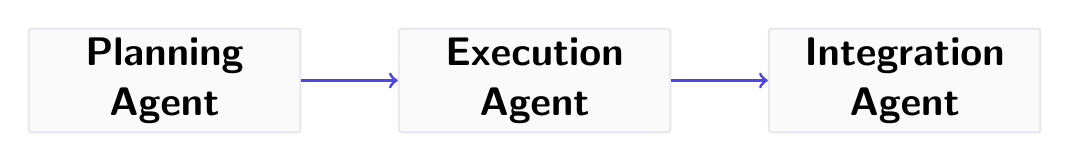
\begin{tikzpicture}[x=1cm,y=1cm]
      \tikzstyle{agent}=[draw=Line, fill=OffWhite, line width=0.7pt, rounded corners=1pt,
        minimum width=3.45cm, minimum height=1.05cm, align=center,
        font=\fontsize{15}{18}\selectfont\bfseries]
      \node[agent] (p) at (0,0) {Planning\\Agent};
      \node[agent] (e) at (4.7,0) {Execution\\Agent};
      \node[agent] (i) at (9.4,0) {Integration\\Agent};
      \draw[->, line width=1.1pt, color=Accent] (p) -- (e);
      \draw[->, line width=1.1pt, color=Accent] (e) -- (i);
    \end{tikzpicture}
  \end{center}

  \vspace{0.35cm}
  \begin{columns}[T,onlytextwidth]
    \begin{column}{0.48\textwidth}
      \compacttext{\textbf{Held constant:} model \protocol{gpt-4o-mini}, temperature 0.3, role prompts, domain-specific max tokens.}
    \end{column}
    \begin{column}{0.48\textwidth}
      \compacttext{\textbf{Manipulated:} the inter-agent communication protocol only.}
    \end{column}
  \end{columns}
\end{frame}

\begin{frame}{Protocols}
  \sectionlabel{EXPERIMENTAL FACTOR}
  \begin{columns}[T,onlytextwidth]
    \begin{column}{0.24\textwidth}
      {\fontsize{20}{25}\selectfont\bfseries NL}\par
      \divider
      \compacttext{Plain English prose, with explicit instruction to avoid structure.}
    \end{column}
    \begin{column}{0.24\textwidth}
      {\fontsize{20}{25}\selectfont\bfseries Markdown}\par
      \divider
      \compacttext{Headings and bullets for readable intermediate reasoning.}
    \end{column}
    \begin{column}{0.24\textwidth}
      {\fontsize{20}{25}\selectfont\bfseries JSON}\par
      \divider
      \compacttext{Validated JSON object with one parse-retry.}
    \end{column}
    \begin{column}{0.24\textwidth}
      {\fontsize{20}{25}\selectfont\bfseries Shared Memory}\par
      \divider
      \compacttext{A blackboard snapshot injected into every downstream agent.}
    \end{column}
  \end{columns}
\end{frame}

\begin{frame}{Experiment}
  \sectionlabel{CONTROLLED GRID}
  \vspace{0.10cm}
  \begin{center}
    \stat{4}{protocols}{NL, Markdown, JSON, Shared Memory}
    \hfill
    \stat{3}{domains}{GSM8K, SQuAD, curated news}
    \hfill
    \stat{360}{pipeline runs}{10 samples x 3 reps per cell}
  \end{center}

  \vspace{0.70cm}
  \begin{columns}[T,onlytextwidth]
    \begin{column}{0.48\textwidth}
      \compacttext{\textbf{Efficiency:} prompt tokens, completion tokens, total tokens, wall-clock latency.}
    \end{column}
    \begin{column}{0.48\textwidth}
      \compacttext{\textbf{Quality:} numeric exact match, SQuAD token-F1, and ROUGE-based news scoring.}
    \end{column}
  \end{columns}
\end{frame}

\begin{frame}{Contributions}
  \sectionlabel{WHAT WE BUILT}
  \begin{enumerate}
    \item \compacttext{Reusable protocol benchmark for a fixed three-agent LLM pipeline.}
    \item \compacttext{360-run dataset with 1,080 message-level logs.}
    \item \compacttext{ANOVA, Tukey HSD, effect sizes, and bootstrap intervals.}
    \item \compacttext{Streamlit demo for protocol recommendations.}
  \end{enumerate}
\end{frame}

\begin{frame}{Token Cost}
  \sectionlabel{RQ1: EFFICIENCY}
  \begin{columns}[T,onlytextwidth]
    \begin{column}{0.61\textwidth}
      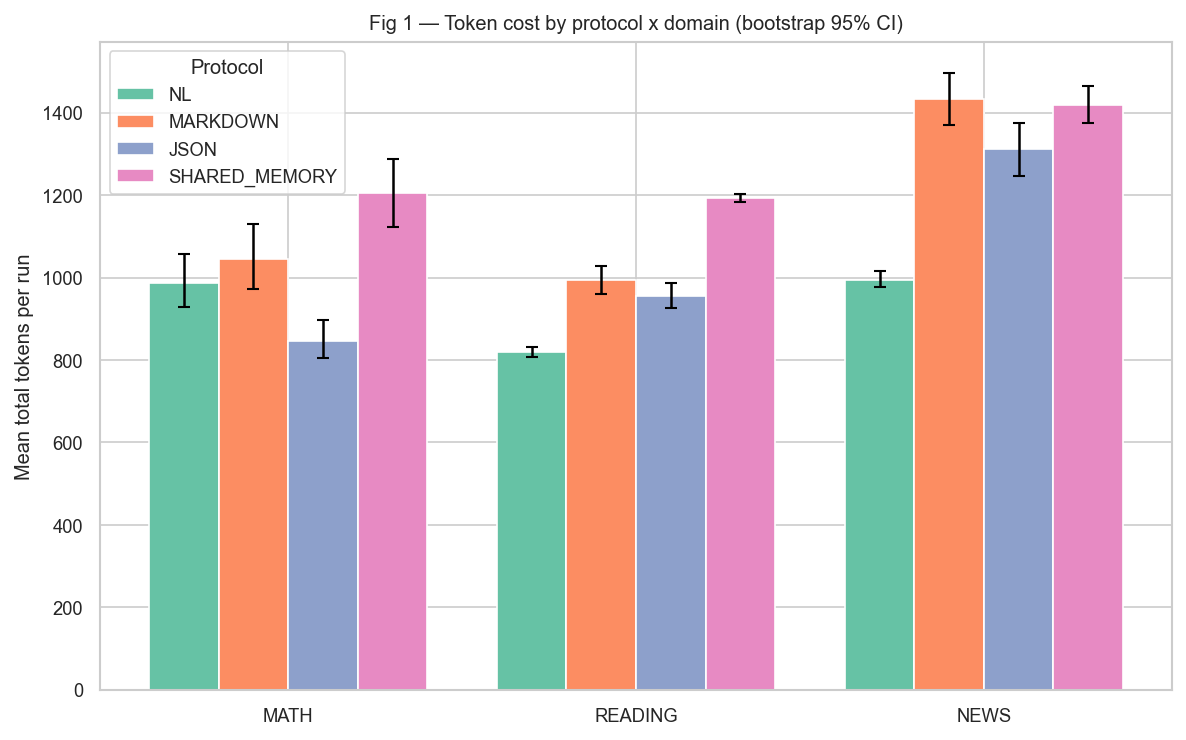
\includegraphics[width=\textwidth,height=0.58\textheight,keepaspectratio]{../figures/fig1_tokens_by_protocol_domain.png}
    \end{column}
    \begin{column}{0.35\textwidth}
      \sidestat{.262}{protocol effect size}{two-way ANOVA on total tokens}\par
      \vspace{0.22cm}
      \compacttext{Shared Memory is the most expensive protocol in every domain: +338 tokens/run versus NL, pooled.}
    \end{column}
  \end{columns}
\end{frame}

\begin{frame}{Where the Tokens Go}
  \sectionlabel{PROMPT VS COMPLETION}
  \begin{columns}[T,onlytextwidth]
    \begin{column}{0.61\textwidth}
      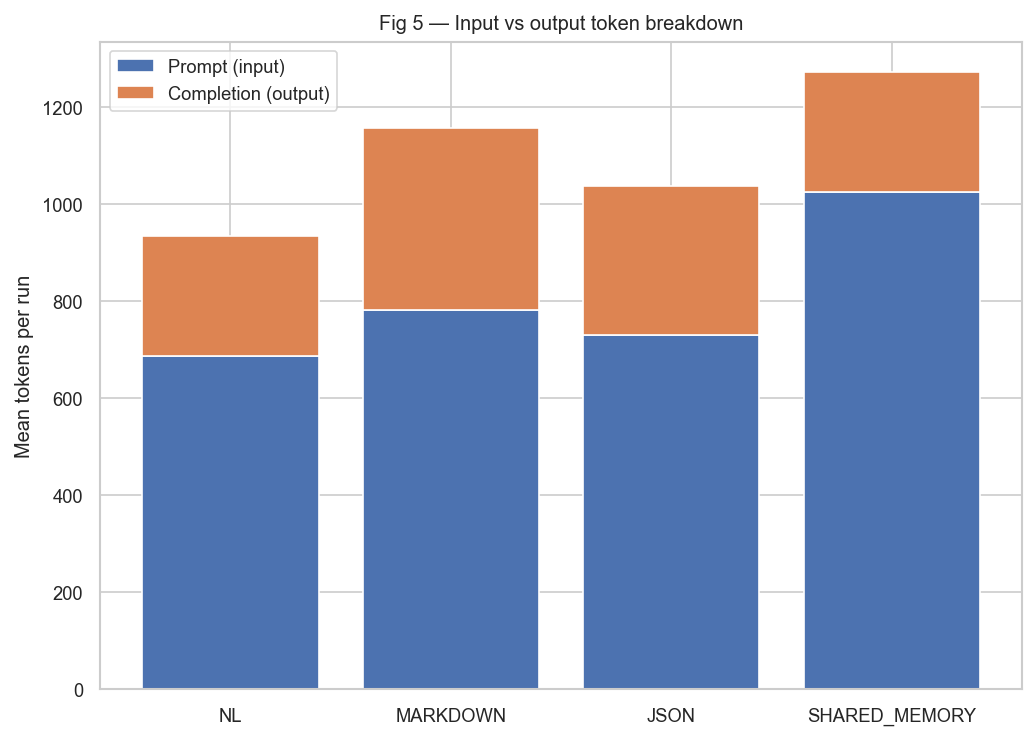
\includegraphics[width=\textwidth,height=0.58\textheight,keepaspectratio]{../figures/fig5_input_vs_output.png}
    \end{column}
    \begin{column}{0.35\textwidth}
      \compacttext{\textbf{Shared Memory} increases prompt tokens: every agent reads the accumulated blackboard.}

      \vspace{0.20cm}
      \compacttext{\hl{Pooled cost order:} NL < JSON < Markdown < Shared Memory.}
    \end{column}
  \end{columns}
\end{frame}

\begin{frame}{Completion Quality}
  \sectionlabel{RQ2: EFFECTIVENESS}
  \begin{columns}[T,onlytextwidth]
    \begin{column}{0.61\textwidth}
      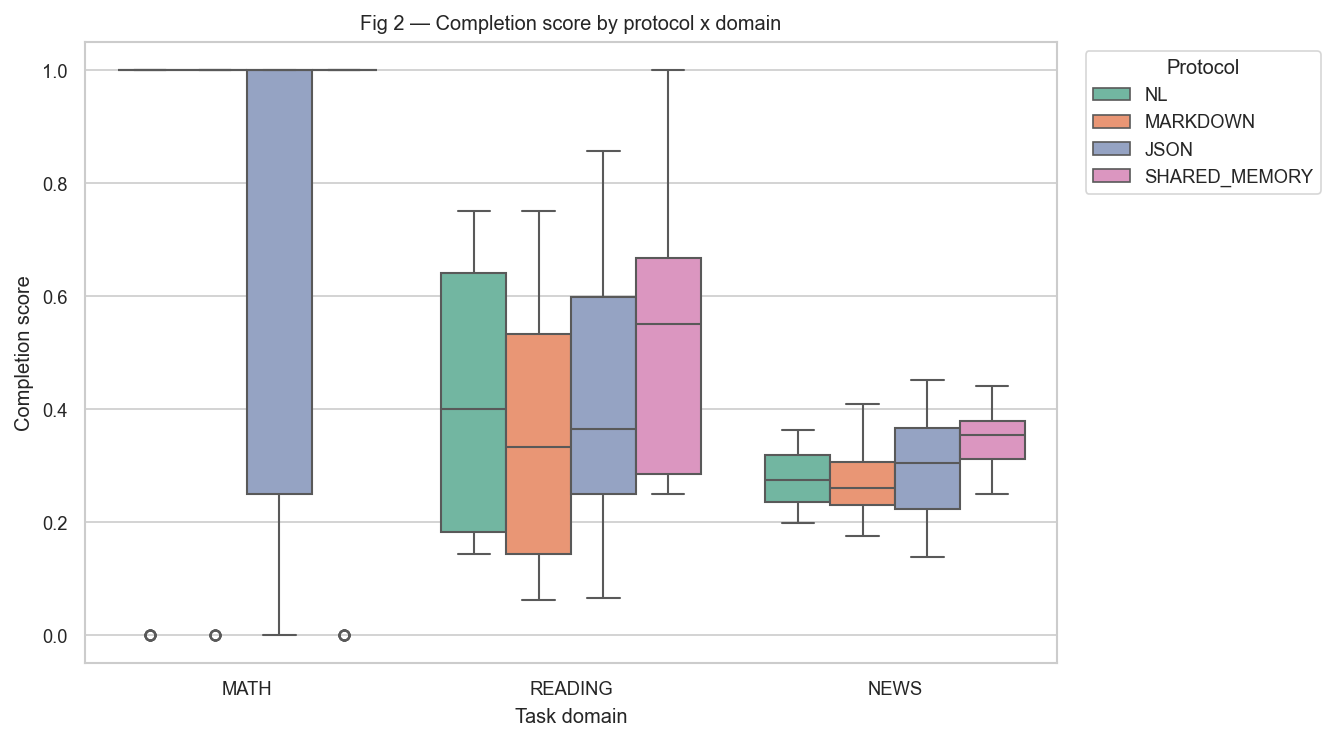
\includegraphics[width=\textwidth,height=0.58\textheight,keepaspectratio]{../figures/fig2_completion_by_cell.png}
    \end{column}
    \begin{column}{0.35\textwidth}
      \sidestat{.017}{math effect size}{protocol mostly changes cost}\par
      \vspace{0.18cm}
      \sidestat{.102}{reading effect size}{Shared Memory leads}\par
      \vspace{0.18cm}
      \sidestat{.197}{news effect size}{largest quality effect}
    \end{column}
  \end{columns}
\end{frame}

\begin{frame}{Domain Interaction}
  \sectionlabel{RQ3: PROTOCOL BY DOMAIN}
  \begin{columns}[T,onlytextwidth]
    \begin{column}{0.60\textwidth}
      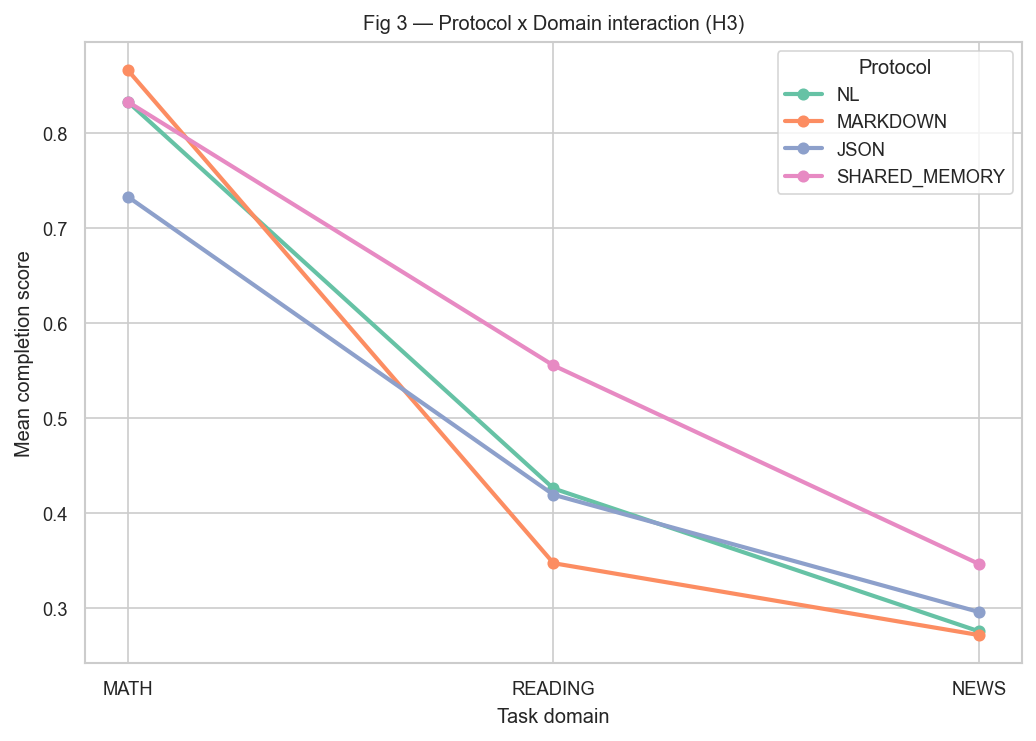
\includegraphics[width=0.96\textwidth,height=0.58\textheight,keepaspectratio]{../figures/fig3_interaction.png}
    \end{column}
    \begin{column}{0.36\textwidth}
      \compacttext{The best protocol changes across domains. Math is flat; reading and news reward richer context.}

      \vspace{0.20cm}
      \compacttext{\hl{Note:} pooled completion interaction: $p=.203$; token interaction: $p<.001$.}
    \end{column}
  \end{columns}
\end{frame}

\begin{frame}{Trade-off}
  \sectionlabel{EFFICIENCY VS EFFECTIVENESS}
  \begin{columns}[T,onlytextwidth]
    \begin{column}{0.60\textwidth}
      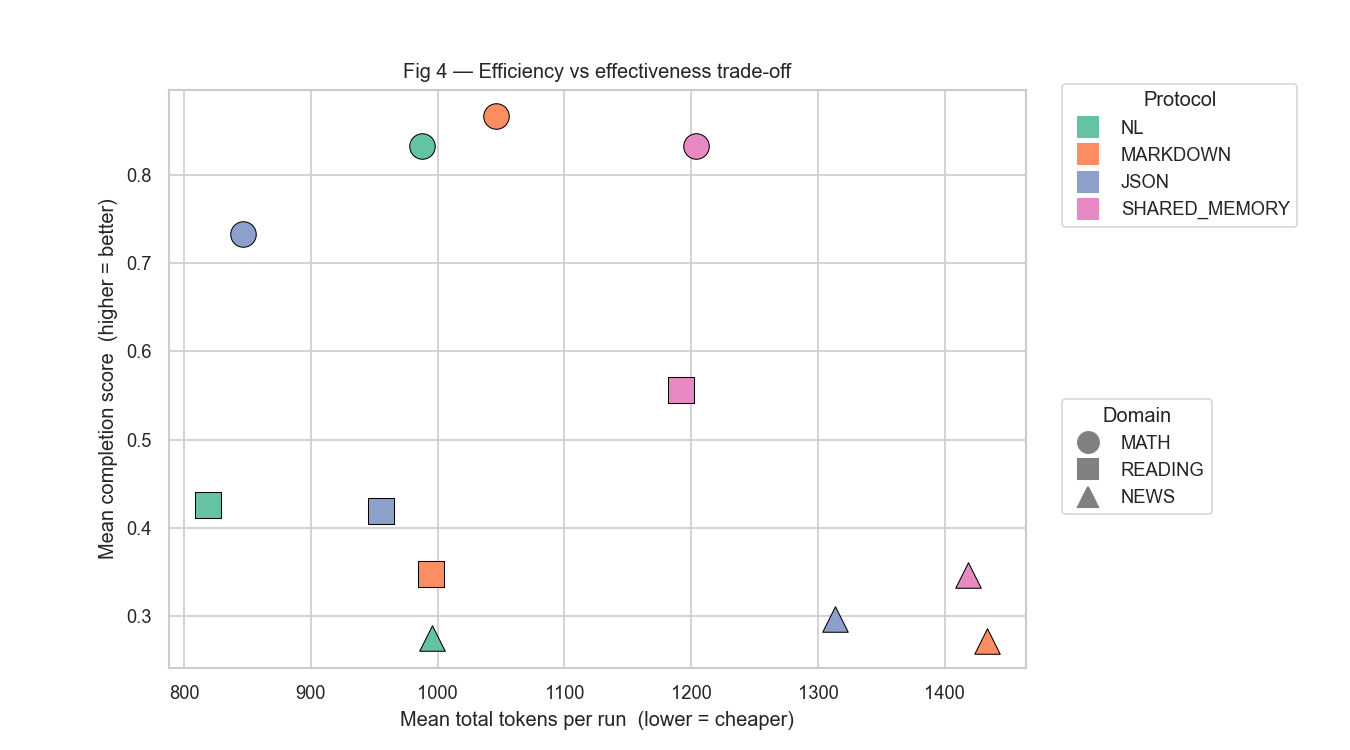
\includegraphics[width=0.98\textwidth,height=0.58\textheight,keepaspectratio]{../figures/fig4_pareto.png}
    \end{column}
    \begin{column}{0.36\textwidth}
      \compacttext{\textbf{Math:} Markdown for best completion; JSON for lowest cost.}

      \vspace{0.30cm}
      \compacttext{\textbf{Reading:} Shared Memory for quality; NL for budget.}

      \vspace{0.30cm}
      \compacttext{\textbf{News:} Shared Memory when factual completeness matters.}
    \end{column}
  \end{columns}
\end{frame}

\begin{frame}{Latency}
  \sectionlabel{OPERATIONAL COST}
  \begin{columns}[T,onlytextwidth]
    \begin{column}{0.61\textwidth}
      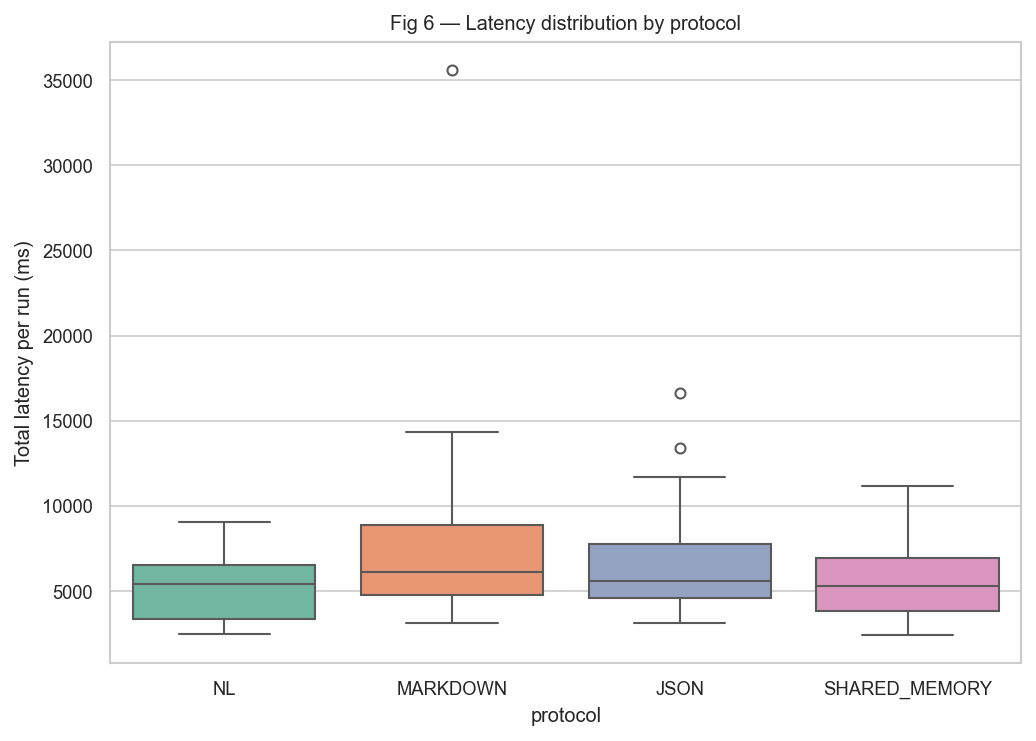
\includegraphics[width=\textwidth,height=0.58\textheight,keepaspectratio]{../figures/fig6_latency.png}
    \end{column}
    \begin{column}{0.35\textwidth}
      \compacttext{Domain complexity dominates latency variance.}

      \vspace{0.35cm}
      \compacttext{Protocol still has a measurable effect: $F=16.55$, $p<.001$, $\eta^2=.070$.}

      \vspace{0.35cm}
      \compacttext{Token-efficient protocols tend to reduce estimated API cost.}
    \end{column}
  \end{columns}
\end{frame}

\begin{frame}{Demo}
  \sectionlabel{PRACTICAL IMPACT}
  \begin{enumerate}
    \item \compacttext{User enters a free-text task.}
    \item \compacttext{The app classifies the task domain.}
    \item \compacttext{It selects the empirically best protocol from \protocol{results\_summary.csv}.}
    \item \compacttext{The pipeline reports tokens, latency, cost, and final answer.}
  \end{enumerate}

  \vspace{0.15cm}
  \compacttext{\hl{Artifact:} single-page Streamlit demo in \protocol{app.py}, with manual protocol override and raw message logs.}
\end{frame}

\begin{frame}{Limitations}
  \sectionlabel{WHAT THIS DOES NOT CLAIM}
  \begin{itemize}
    \item \compacttext{Only 10 samples per domain and 3 repetitions per cell.}
    \item \compacttext{All agents use \protocol{gpt-4o-mini}; effects may differ under other models.}
    \item \compacttext{Three-agent chain only, not branching debate or tool workflows.}
    \item \compacttext{Future work: larger samples, hybrid protocols, heterogeneous agents, dynamic switching.}
  \end{itemize}
\end{frame}

\begin{frame}{Takeaways}
  \sectionlabel{FINAL RECOMMENDATION}
  {\fontsize{24}{30}\selectfont\bfseries
  Do not choose an agent communication protocol globally. Choose it by domain and by whether the priority is cost or completion quality.}

  \vspace{0.45cm}
  \begin{columns}[T,onlytextwidth]
    \begin{column}{0.31\textwidth}
      \compacttext{\hl{Cost:} NL and JSON are strong budget choices.}
    \end{column}
    \begin{column}{0.31\textwidth}
      \compacttext{\hl{Quality:} Shared Memory helps reading and news.}
    \end{column}
    \begin{column}{0.31\textwidth}
      \compacttext{\hl{Artifact:} code, results, figures, and demo are reproducible.}
    \end{column}
  \end{columns}
\end{frame}

\begin{frame}{Backup: Cell Summary}
  \sectionlabel{RESULTS SUMMARY, N=30 PER CELL}
  \vspace{-0.08cm}
  \begin{table}
    \centering
    \fontsize{8.8}{10.8}\selectfont
    \begin{tabular}{llrrrr}
      \toprule
      Protocol & Domain & Tokens & Prompt & Completion & Score \\
      \midrule
      \protocol{NL} & Math & 988 & 665 & 323 & .833 \\
      \protocol{NL} & Reading & 819 & 717 & 102 & .426 \\
      \protocol{NL} & News & 995 & 680 & 315 & .275 \\
      \protocol{Markdown} & Math & 1046 & 695 & 351 & .867 \\
      \protocol{Markdown} & Reading & 995 & 794 & 201 & .347 \\
      \protocol{Markdown} & News & 1433 & 860 & 574 & .271 \\
      \protocol{JSON} & Math & 847 & 600 & 247 & .733 \\
      \protocol{JSON} & Reading & 955 & 777 & 178 & .419 \\
      \protocol{JSON} & News & 1313 & 815 & 498 & .296 \\
      \protocol{Shared Memory} & Math & 1204 & 931 & 273 & .833 \\
      \protocol{Shared Memory} & Reading & 1192 & 1095 & 97 & .556 \\
      \protocol{Shared Memory} & News & 1418 & 1052 & 366 & .346 \\
      \bottomrule
    \end{tabular}
  \end{table}
  \smallmuted{Source: results/results\_summary.csv}
\end{frame}

\end{document}
